\documentclass[9pt,twocolumn,twoside,pdftex]{optica}
\setboolean{shortarticle}{false}
\setboolean{minireview}{false}


\title{Dual oxygen and temperature sensing multi-task learning neural networks}

\author[1,2,*]{Francesca Venturini}
\author[2]{Umberto Michelucci}
\author[1]{Michael Baumgartner}

\affil[1]{Institute of Applied Mathematics and Physics, Zurich University of Applied Sciences,
Technikumstrasse 9, 8401 Winterthur, Switzerland}
\affil[2]{TOELT LLC; Birchlenstr. 25, 8600 Dübendorf, Switzerland}

\affil[*]{Corresponding author: francesca.venturini@zhaw.ch}

% To be edited by editor
% \dates{Compiled \today}

%\ociscodes{(140.3490) Lasers, distributed feedback; (060.2420) Fibers, polarization-maintaining; (060.3735) Fiber Bragg gratings.}
%300.6280   Spectroscopy, fluorescence and luminescence
%260.3800   Luminescence
%120.0280   Remote sensing and sensors
%100.4996   Pattern recognition, neural networks
%200.4260   Neural networks
%https://www.osapublishing.org/submit/ocis/#230.0230
% To be edited by editor
% \doi{\url{http://dx.doi.org/10.1364/optica.XX.XXXXXX}}

\begin{abstract}

A well-known optical approach to measure oxygen partial pressure is the quenching of luminescence by the oxygen molecules. Sensors based on this principle typically rely on approximate empirical models to parametrise the dependence of the sensing quantity on influencing factors, like the temperature. In this work, we propose a new multi-task learning (MTL) neural network approach which allows the extraction of both the oxygen concentration and the temperature using one single indicator and measuring a single quantity, namely the decay time. The results demonstrate that firstly, using neural networks it is possible to extract both the oxygen concentration and the temperature from the measurement of one single quantity and using one single indicator; secondly, that the use the proposed MTL networks allow more accurate and stable predictions for both the parameters. Furthermore, the proposed MTL approach is not limited to luminescence quenching but paves the way for applications where the mathematical model is not known, too complex or not really of interest.


\end{abstract}

\setboolean{displaycopyright}{true}

\begin{document}

\maketitle

\section{Introduction}

The determination of oxygen partial pressure is of great interest in numerous areas, like medicine, biotechnology, and chemistry. Among the different methods used to determine oxygen concentration, optical techniques are particularly attractive because they do not consume oxygen, have a fast response time, allow a good precision and accuracy. A well-known optical measuring approach is the quenching of luminescence by the oxygen molecules. The measuring principle is based on the measurement of the luminescence of a specific molecule, whose intensity and the decay time are reduced due to collisions with oxygen. Sensors based on this principle typically rely on approximate empirical models to parametrise the dependence of the sensing quantity on influencing factors. A new approach is to use feed-forward neural networks to predict the desired variables. Unfortunately, those kind of networks usually perform less efficiently when applied to multi-dimensional regression problems. In this work, we propose a new multi-task learning (MTL) neural network approach which allows the extraction of both the oxygen concentration and the temperature using one single indicator and measuring a single quantity, namely the decay time. The results demonstrate that firstly, using neural networks it is in principle possible to extract both the oxygen concentration and the temperature from the measurement of one single quantity and using one single indicator; secondly, that the use the proposed MTL networks allow more accurate and stable predictions for both the parameters. Furthermore, the proposed MTL approach is not limited to luminescence quenching but may be of particular relevance in all those cases, where the mathematical model is not known, too complex or not really of interest and the only goal of the regression problem is to build a system that is able to determine as accurately as possible..

\section{Methods}
\label{sec:methods}

\subsection{Theoretical model for Luminescence Quenching for Oxygen Determination}
\label{Theory}

\subsection{Experimental Setup}
\label{Experimental}

The sample used for the characterization and test is a commercially available Pt-TFPP-based oxygen sensor spot (PSt3, PreSens Precision Sensing GmbH).
To control the temperature of the samples, these were placed in good thermal contact with a copper plate, placed in a thermally insulated chamber. The temperature of this plate was adjusted at a fixed value between 5 $^\circ$C and 45 $^\circ$C in 5 $^\circ$C steps using a Peltier element and stabilized with a temperature controller (PTC10, Stanford Research Systems). The thermally insulated chamber was connected to a self-made gas-mixing apparatus which enabled to vary the oxygen concentration between 0 $\%$ and 20 $\%$ vol $O_2$ by mixing nitrogen and dry air from two bottles. In the following, the concentration of oxygen will be given in $\%$ of the oxygen concentration of dry air and indicated with $\%$ air. This means, for example, that 20 $\%$ air corresponds to 4 $\%$ vol $O_2$ and 100 $\%$ air corresponds to 20 $\%$ vol $O_2$. The absolute error on the oxygen concentration adjusted with the gas mixing device is estimated to be below 1 $\%$ air. The oxygen concentration was varied between 0 $\%$ air and 100 $\%$ air in 5 $\%$ steps.
 
The optical setup used in this work for the luminescence measurements is shown schematically in Fig. \ref{fig:setup}.

\begin{figure}[htbp]
\centering
\includegraphics[keepaspectratio, width=8.5cm]{setup_auto.eps}
\caption{Scheme of the optical experimental setup. Blue is the excitation, red the luminescence optical path. PD: photodiode; TIA: trans-impedance amplifier.}
\label{fig:setup}
\end{figure}
The excitation light was provided by a 405 nm LED (VAOL-5EUV0T4, VCC Visual Communications Company LLC), filtered by a an short pass (SP) filter with cut-off at 498 nm (Semrock 498 SP Bright Line HC short pass) and focused on the surface of the samples with a collimation lens (EO43987, Edmund Optics). The luminescence was focussed by a lens (G063020000, LINOS) and collected by a photodiode (SFH 213 Osram).
To suppress stray light and light reflected by the sample surface, the emission channel was equipped with a long pass filter with cut-off at 594 nm (Semrock 594 LP Edge Basic long pass) and a short pass filter with cut-off at 682 nm (Semrock 682 SP Bright Line HC short pass). The driver for the LED and the trans-impedance amplifier (TIA) are self-made.
For the frequency generation and the phase detection a two-phase lock-in amplifier (SR830, Stanford Research Inc.) was used. The modulation frequency was varied between 200 Hz and 15000 kHz.

\subsection{Automated Data Acquisition}
\label{Data}

The series of measurements were carried out following the flow shown in Fig. XXX. First the acquisition program fixed the temperature and concentration. Then the phase-shift was measured for varying the modulation frequency. This measurement was repeated 20 times. Next, keeping the temperature fixed, the program changed the oxygen concentration and the entire frequency-loop was repeated. Finally, the temperature is changed and then the oxygen and frequency loops where repeated.
The total number of measurements is 50x20x21x9=189000 which lasted ca. 65 hours. The number of measurement was chosen as a compromise between maximal number of measurements and minimal change of the sample due to photobleaching. 

\begin{figure}[htbp]
\centering
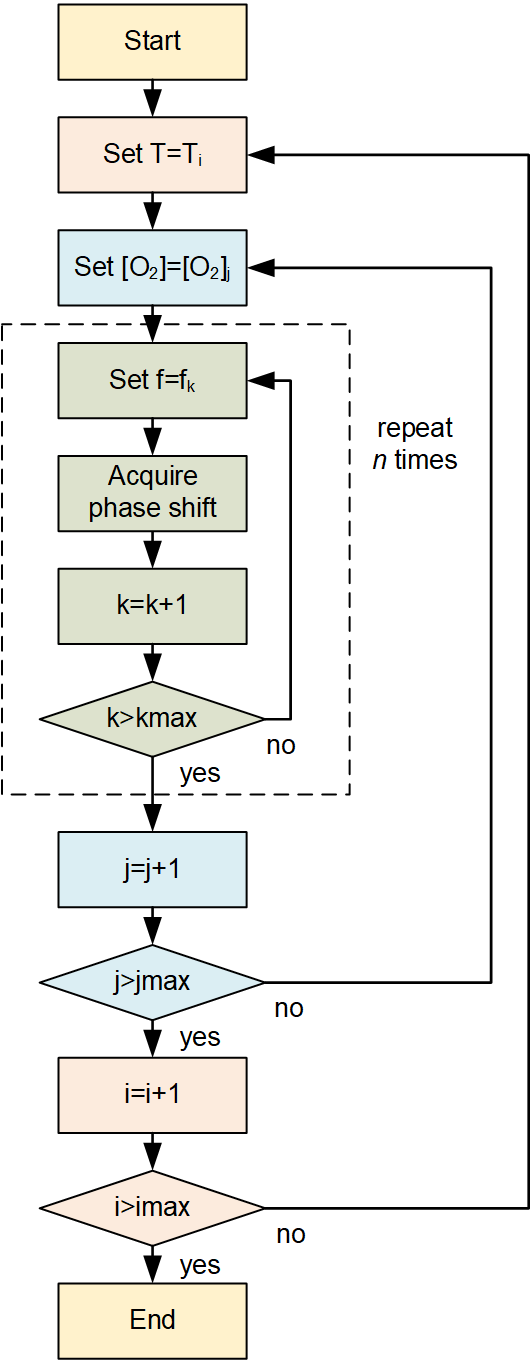
\includegraphics[keepaspectratio, width=5 cm]{flow-chart.png}
\caption{Scheme of the optical experimental setup. Blue is the excitation, red the luminescence optical path. PD: photodiode; TIA: trans-impedance amplifier.}
\label{fig:setup}
\end{figure}

\subsection{Artificial Neural Network Design}
\label{NN}

The MTL network proposed is depicted in Figure \ref{fig:NN_MTL_O2_T}. It consists of three common hidden layers with 50 neurons each which generate as output a "shared representation". The name comes from the fact that the output of those layers is used to evaluate both $[O_2]$ and $T$. These are followed by three branches, two with each two additional "task-specific hidden layers" to predict respectively $[O_2]$ and $T$, and then one without additional layers to predict $[O_2]$ and $T$ at the same time.The shared representation is the input of two "task-specific hidden layers", that learn how to predict $[O_2]$ and $T$ better. Note how the common hidden layers are shared with both the tasks of predicting $[O_2]$ and $T$, while the task-specific hidden layers are specific to each task separately. Therefore, the MTL  network uses the common hidden layers to find common features beneficial to each of the two tasks. During the training phase, learning to predict $[O_2]$ will influence the common hidden layers and therefore, the prediction of $T$, and vice-versa. A set of task-specific hidden layers will then learn specific features to each output and therefore improve the prediction accuracy.
The number of neurons of each task-specific hidden layer is 5.

In the three architectures investigated the sigmoid activation functions was used for all the neurons.

A common choice for the cost function in regression problems is the mean square error (MSE), which is defined as
\begin{equation}
MSE = \frac{1}{n}\sum_{j=1}^n \sum_{k=1}^d (y_k^{[j]}-\hat y_k^{[j]})^2
\label{MSE}
\end{equation}
where $n$ is the number of observations in the input dataset; ${\mathbold y}^{[j]} \in \mathbb{R}^d$ is the measured value of the desired quantity for the $j^{th}$ observation (indicated as a superscript between square brackets), with $j=1, ..., n$; $ \hat {\mathbold y}^{[j]} \in \mathbb{R}^d$ is the output of the network, when evaluated on the $j^{th}$ observation.T Since there are multiple branches, a global cost function $L$ needs to be defined as a linear combination of the task-specific cost functions with weights $\alpha_i$ will be minimized
\begin{equation}
L = \sum_{i=1}^{n_T}\alpha_i L_i .
\label{globalcf}
\end{equation}
The parameters $\alpha_i$ have to be determined during the hyper-parameter tuning phase to optimize the network predictions.
In this paper, being the cost function the MSE (Equation \ref{MSE}), the global cost function of Equation \ref{globalcf} is
\begin{equation}
L = \sum_{i=1}^{n_T}\alpha_i \frac{1}{n}\sum_{j=1}^n \sum_{k=1}^d (y_k^{[j]}-\hat y_k^{[j]})^2
\end{equation}
where  $n_T$ is the number of tasks; $n$ is the number of observations in the input dataset; ${\mathbold y}^{[j]} \in \mathbb{R}^d$ is the measured value of the desired quantity for observation $j$, with $j=1, ..., n$; $ \hat {\mathbold y}^{[j]} \in \mathbb{R}^d$ is the output of the network, when evaluated on the $j^{th}$ observation.
he global cost function weights used for the plots were $\alpha_1 = 0.3$, $\alpha_2 = 5$ and $\alpha_3 = 1$. Those values were chosen because they result in the lowest $MAE$s (see discussion in Section \ref{Results}).
 

\begin{figure}[htbp]
\centering
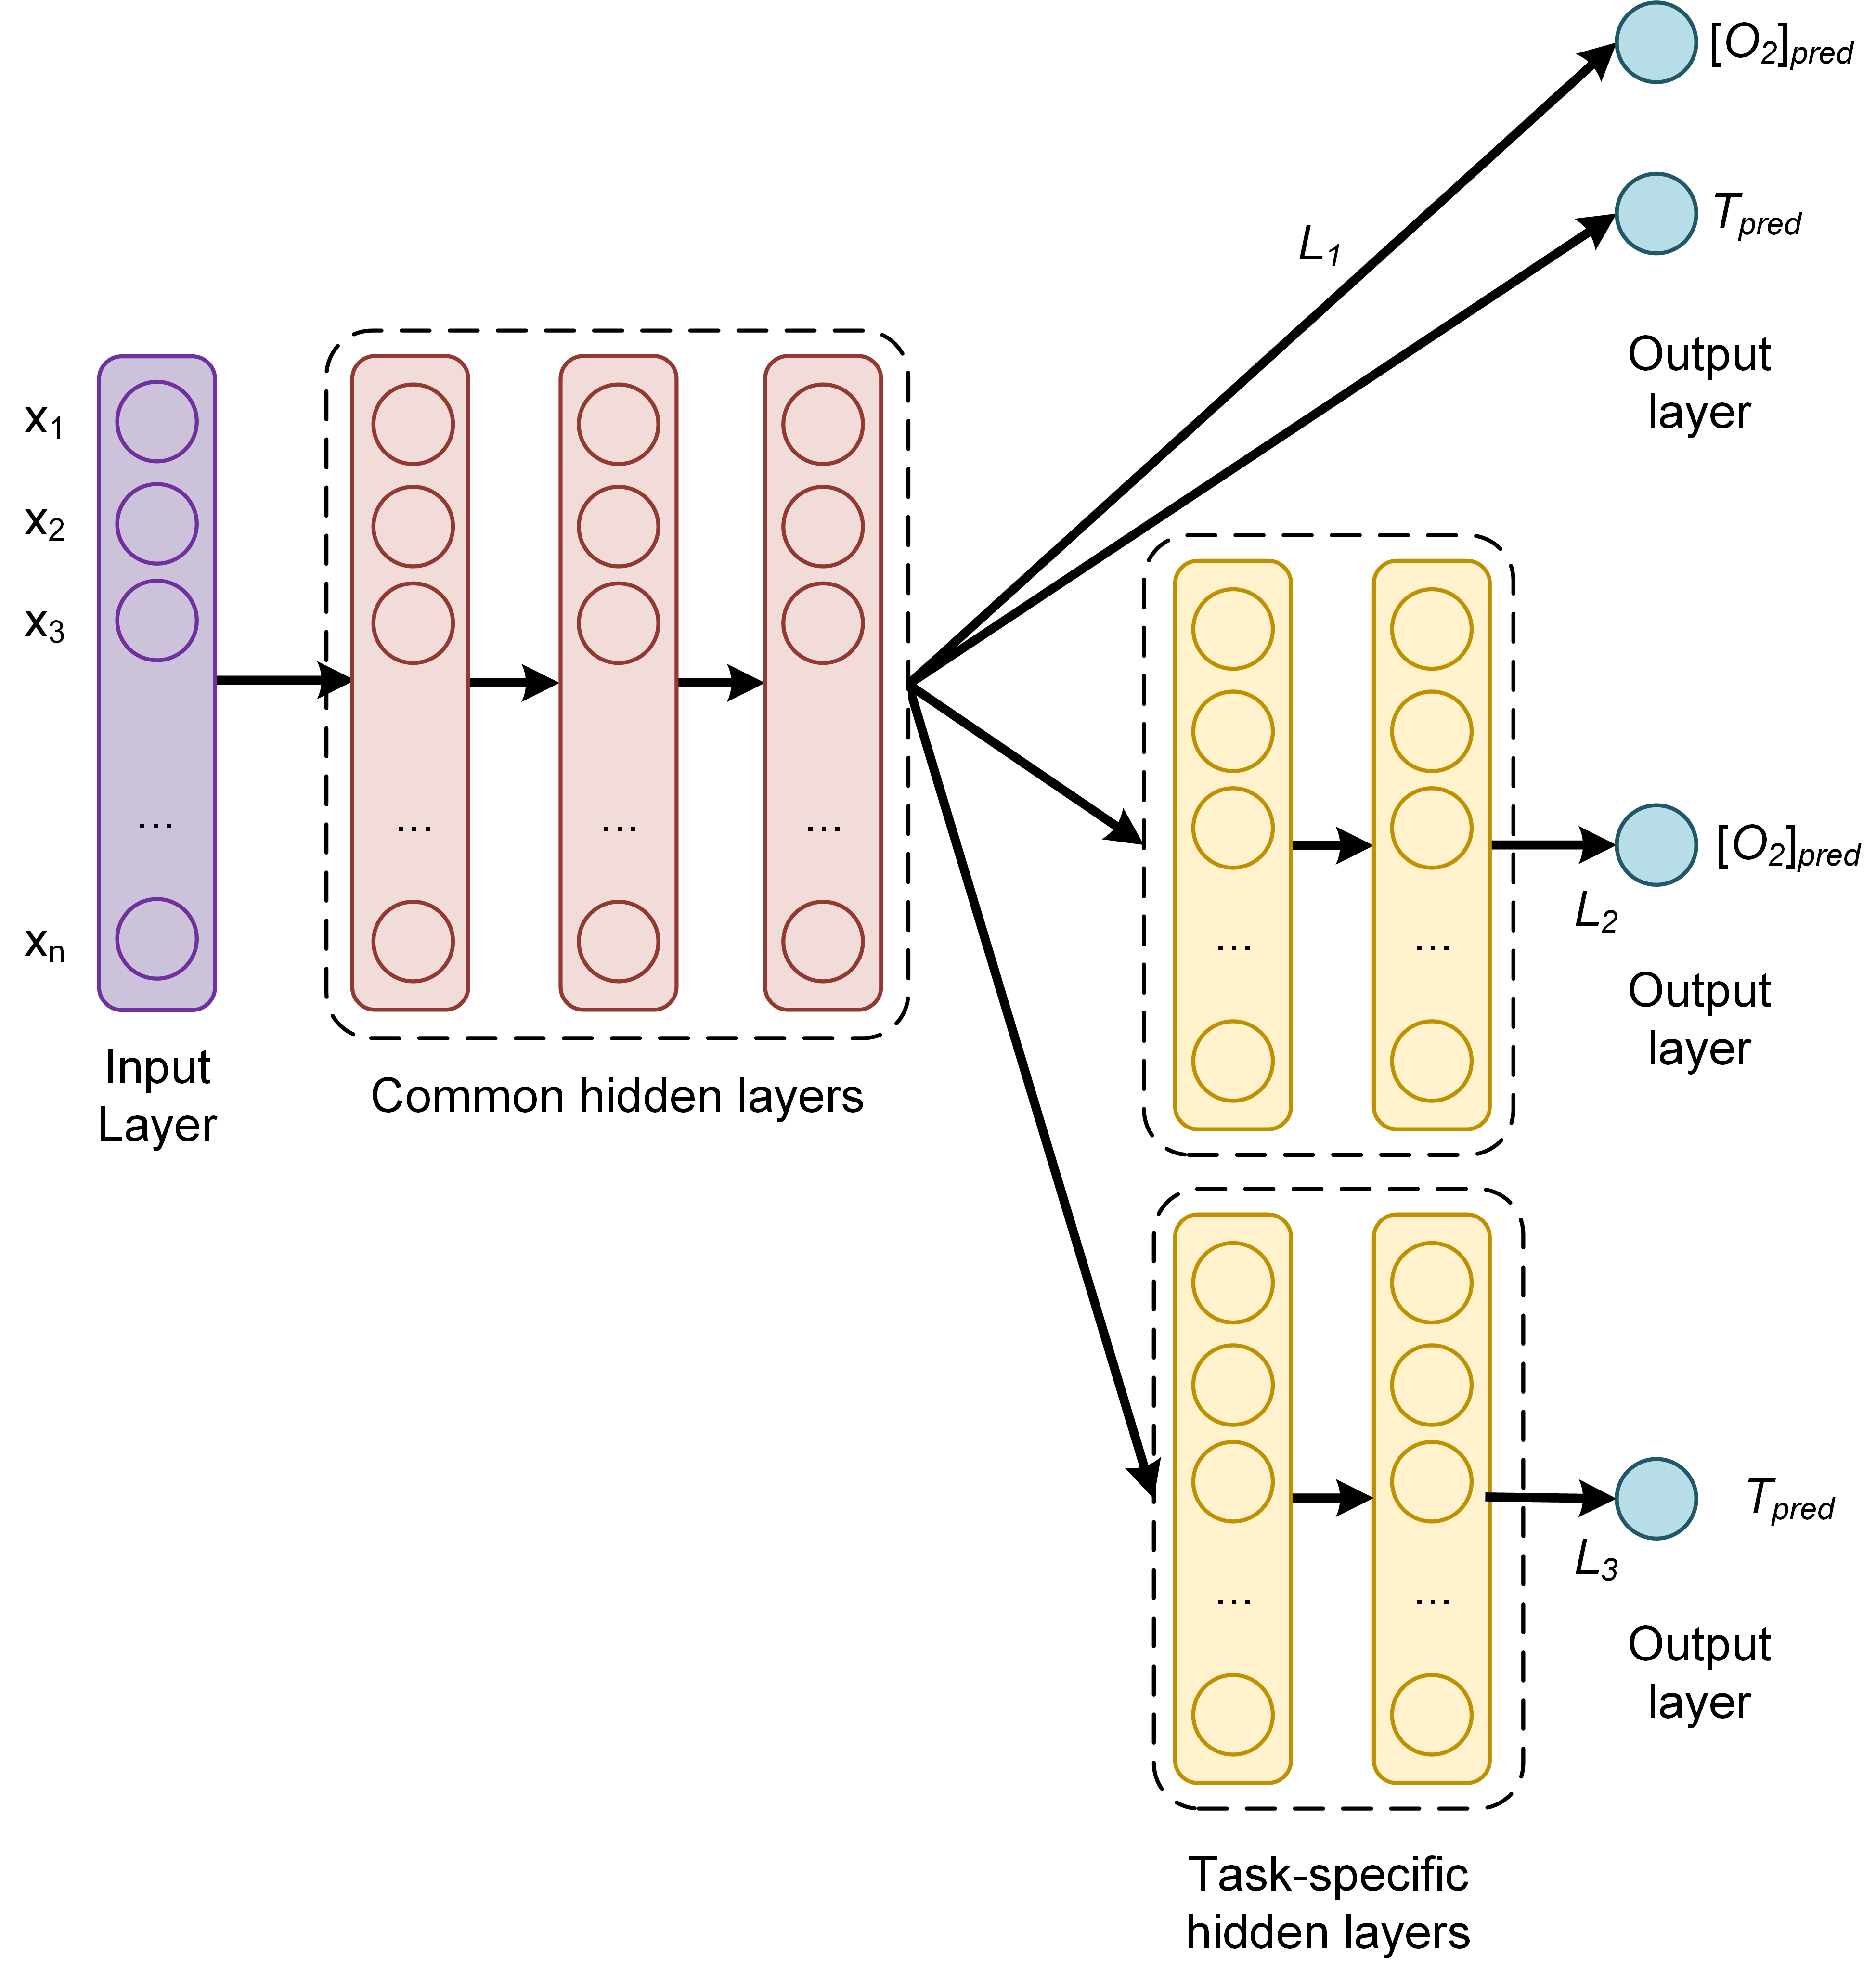
\includegraphics[width=9 cm]{NN_MTL_O2_T.png}
\caption{Architecture of the feed-forward MTL.}
\label{fig:NN_MTL_O2_T}
\end{figure}

To minimize the cost function, the optimizer Adaptive Moment Estimation (Adam) \cite{Kingma2014, Michelucci2017} was used. The training was performed with a starting learning rate of $10^{-3}$ and using batch-learning, which means that the weights were updated only after the entire training dataset has been fed to the network. Batch-learning was chosen because of its stability and speed since it reduces the training time of a few orders of magnitude in comparison to, for example, stochastic gradient descent \cite{Michelucci2017}. Therefore it makes experimenting with different networks a feasible endeavor. 
The implementation was performed using the TensorFlow$\texttrademark$ library. 

The metric used to compare results from different network models is the 
absolute error ($AE$) defined as the absolute value of the difference between the predicted and the expected value for a given observation. For the oxygen concentration of the 
$j^{th}$ observation $[O_2]^{[j]}$  the $AE$ is 
\begin{equation}
\label{AE}
AE^{[j]}_{[O_2]} = |[O_2]^{[j]}_{pred}-[O_2]^{[j]}_{meas}|.
\end{equation}

The further quantity used to analyze the performance of the network is the mean absolute error ($MAE$), defined as the average of the absolute value of the difference between the predicted and the expected oxygen concentration or temperature. For example, for the oxygen prediction using the training dataset $S_{train}$, $MAE_{[O_2]}$ is defined as 
\begin{equation}
\label{MAE}
MAE_{[O_2]}(S_{train}) = \frac{1}{|S_{train}|} \sum_{j \in S_{train}}|[O_2]_{pred}^{[j]}-[O_2]_{real}^{[j]}|
\end{equation}
where $|S_{train}|$ is the size (or cardinality) of the training dataset. For example, in this work $|S_{train}|$=20000.
The $AE_{T}$ and $MAE_T$ are similarly defined.

\section{Results and Discussion}
\ref{Results}

\begin{figure}[htbp]
\centering
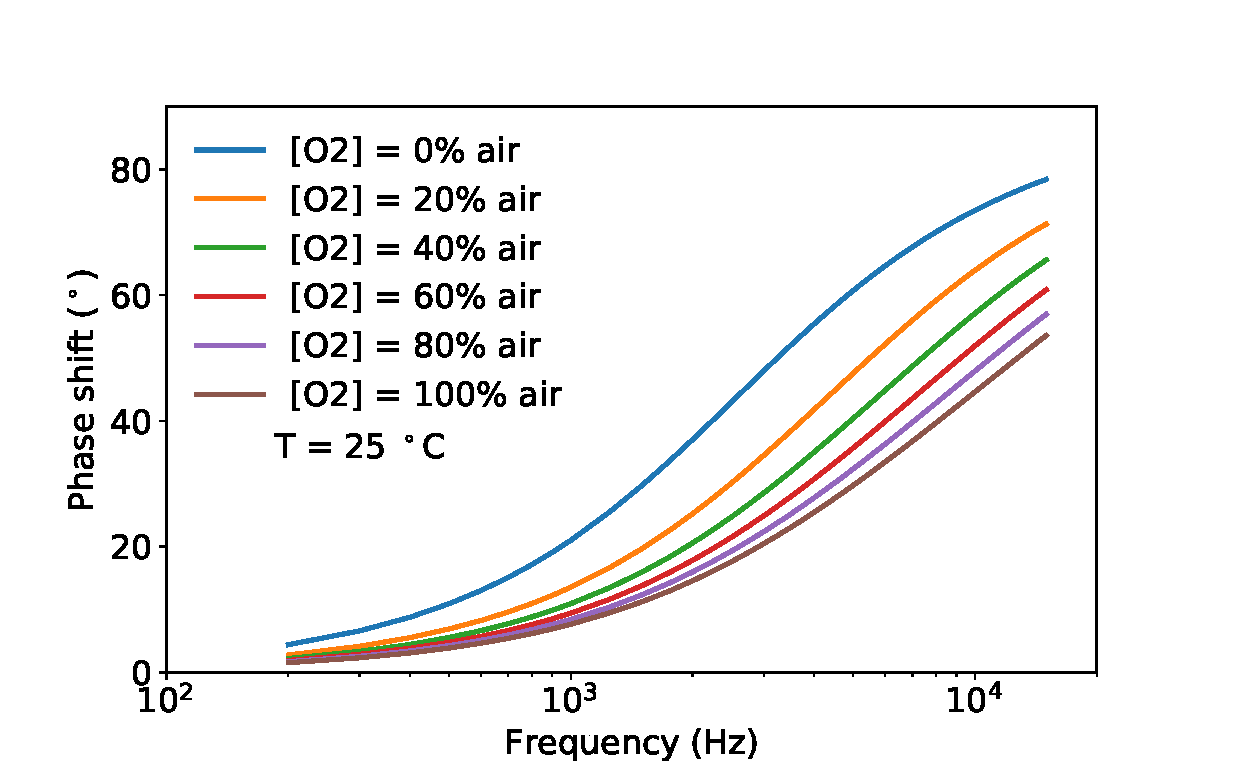
\includegraphics[width=9 cm]{expdata1.eps}
\caption{At temperature 25....}
\label{fig:expdata1}
\end{figure}

\begin{figure}[htbp]
\centering
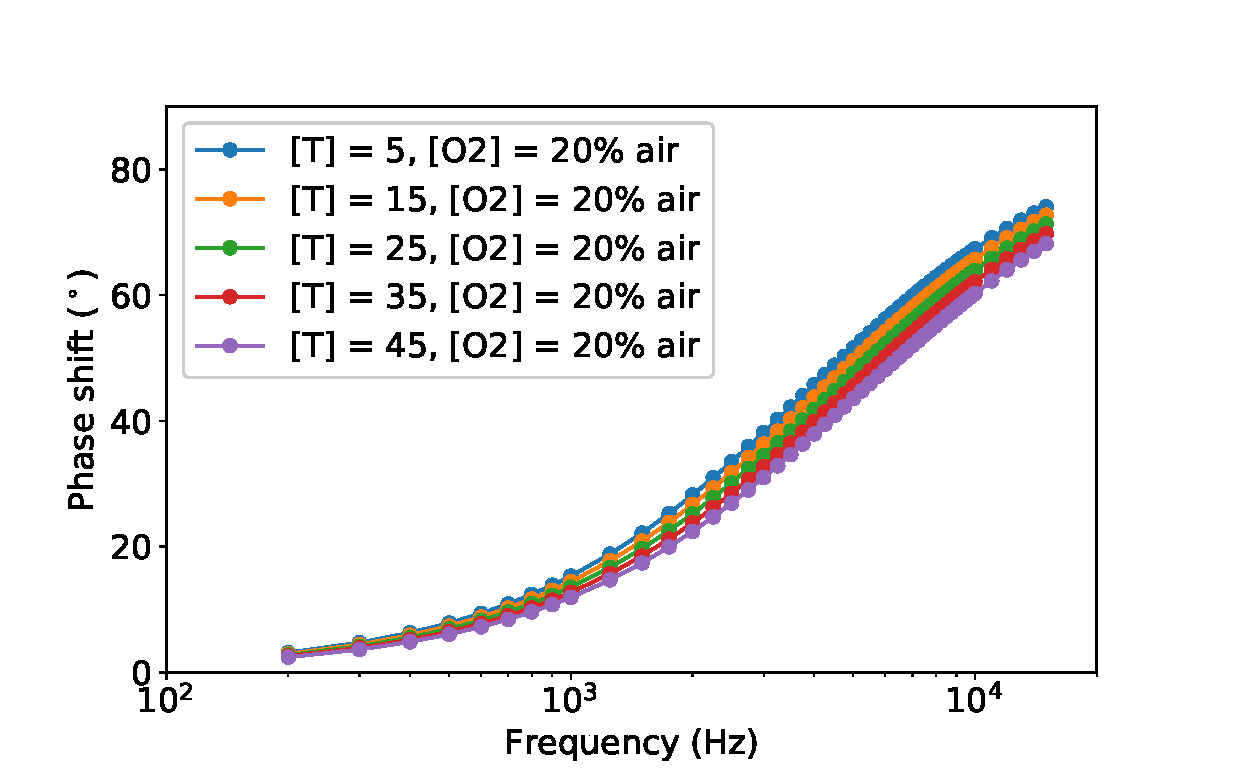
\includegraphics[width=9 cm]{expdata2.eps}
\caption{....}
\label{fig:expdata2}
\end{figure}
\subsection{Sample Table}

Table \ref{tab:shape-functions} shows an example table.

\begin{table}[htbp]
\centering
\caption{\bf Shape Functions for Quadratic Line Elements}
\begin{tabular}{ccc}
\hline
local node & $\{N\}_m$ & $\{\Phi_i\}_m$ $(i=x,y,z)$ \\
\hline
$m = 1$ & $L_1(2L_1-1)$ & $\Phi_{i1}$ \\
$m = 2$ & $L_2(2L_2-1)$ & $\Phi_{i2}$ \\
$m = 3$ & $L_3=4L_1L_2$ & $\Phi_{i3}$ \\
\hline
\end{tabular}
  \label{tab:shape-functions}
\end{table}


\section{Conclusions}



%\section*{Funding Information}
%National Science Foundation (NSF) (1263236, 0968895, 1102301); The 863 Program (2013AA014402).

%\section*{Acknowledgments}


\section*{Disclosures}

\medskip

\noindent\textbf{Disclosures.} The authors declare no conflicts of interest.

\section*{Supplemental Documents}
\emph{Optica} authors may include supplemental documents with the primary manuscript. For details, see \href{http://www.opticsinfobase.org/submit/style/supplementary-materials-optica.cfm}{Supplementary Materials in Optica}. To reference the supplementary document, the statement ``See Supplement 1 for supporting content.'' should appear at the bottom of the manuscript (above the references).

%\bigskip \noindent See \href{link}{Supplement 1} for supporting content.

\section*{References}

For references, you may add citations manually or use BibTeX. E.g. \cite{Michelucci2017}.

Letter submissions to \emph{Optica} require two sets of references: an abbreviated reference style for publication and a full reference list to aid the editor and reviewers. Citations to journal articles in the abbreviated list should omit the article title and final page number; this abbreviated reference style is produced automatically when the \texttt{$\setminus$setboolean\{shortarticle\}\{true\}} option is selected in the template, if you are using a .bib file for your references.
 
The full reference list meant to aid the editor and reviewers must be included as well on an informational page that will not count against page length; again this will be produced automatically if you are using a .bib file and have the \texttt{$\setminus$setboolean\{shortarticle\}\{true\}} option selected.


% Bibliography
\bibliography{bibliography}

% Full bibliography will be added automatically on a new page for Optics Letters submissions. This command is ignored for journal article submissions.
% Note that this extra page will not count against page length.
\bibliographyfullrefs{bibliography}

%\printbibliography

%Manual citation list
%\begin{thebibliography}{1}
%\bibitem{Michelucci2017}
%Michelucci, U.
%{\sl Applied Deep Learning - A Case-Based Approach to Understanding Deep Neural Networks}; Apress Media, LLC: New York, NY, USA, 2018; pp. 374--375.

%\bibitem{Kingma2014}
%Kingma, D.P.; Ba, J.
%Adam: A method for stochastic optimization. In Proceedings of 3rd International Conference on Learning Representations, ICLR 2015, San Diego, CA, USA, May 7-9, 2015, pp. 1--15.

%\bibitem{Michelucci2019}
%Michelucci, U.; Baumgartner, M.; Venturini, F.
%Optical oxygen sensing with artificial intelligence.
%{\sl Sensors} {\bf 2019}, {\sl 19}, 777.

˜
%\bibitem{Zhang:14}
%Y.~Zhang, S.~Qiao, L.~Sun, Q.~W. Shi, W.~Huang, %L.~Li, and Z.~Yang,
 % \enquote{Photoinduced active terahertz metamaterials with nanostructured
  %vanadium dioxide film deposited by sol-gel method,} Opt. Express \textbf{22},
  %11070--11078 (2014).
%\end{thebibliography}

\end{document} 